\section{ELSE}
Um die Blickrichtung möglichst exakt zu bestimmen, sind die Landmarks der Pupille ausschlaggebend. Zu diesem Zwick kann ElSe eingesetzt werden, da dies ein Verfahren zur Detektion von Pupillen in Bildern unter realen Bedingungen ist.
\subsection{Funktion}
Das Verfahren ist in der Lage aus Bildern die Umrisse einer Pupille zu ermitteln. Bei realen Aufnahmen sind Bildfehler unvermeidlich, es können Reflektionen (Brille, Kontaktlinse usw.) Make-Up oder körperliche Eigenschaften wie Augenfarbe auftreten um die Detektion erschweren.\\
Als Ergebnis liefert ElSe eine Ellipse, die den Umriss der Pupille beschreibt.
\subsection{Funktionsablauf}
Als Input wird im Orginal ein Graubild verwendet, auf dem das Infrarot beleuchtete Auge abgebildet ist. Für den Test im Vergleich zu anderen Verfahren, wurden Bilder von $384\times 288$ Pixel Größe verwendet und ist auf diesen Echtzeit fähig.
\subsubsection{Kantendetektion}
Da die Pupille als schwarzen Fleck sichtbar ist und die Iris einen helleren Farbton aufweist, wird ein Kantendetektor verwendet, der alle Pixel markiert, bei denen eine starke Farbänderung auftritt. Bei ElSe wird ein Morphologischen Ansatz eingesetzt, von Relevanz sind nur zusammenhängende Kantenpixel, alle anderen können ignoriert werden.
\subsubsection{Bestimmen der Ellipse}
Um jene Kantenpixel zu erhalten, die die Pupille beschreiben, wird versucht fortlaufende Kanten zu finden, die eine Ellipse bilden. Jene die nicht diesen Anforderung entsprechen können recht schnell ignoriert werden. Anschließend können auch alle offenen Ellipsenverläufe und jene die am meisten vom bestimmten Verlauf abweichen, verworfen werden.\\
Das beste Ergebnis aller so bestimmten Ellipsen, wird als Lösung verwendet.
\subsubsection{Grobe Bestimmung}
Sollte die Bestimmung der Ellipse scheitern, so wird das Zentrum des dunkelsten Kreises ermittelt, so ein Punkt kann immer gefunden werden, ist aber nicht zwingend die Pupille.\\
Auf einem verkleinertem Bild \autoref{img_else} (1) wird ein kreisförmiger Mean-Filter eingesetzt mit Ergebnis \autoref{img_else} (3). Zur zweiten Faltung mit Ergebnis \autoref{img_else} (2) wir der negative Durchschnitt über ein Quadrat ohne inneren Kreis eingesetzt, wobei der Mean- und negativen Mean-Filter den selbe Radius haben.\\
Nun wird das Ergebnis des Mean-Filters invertiert \autoref{img_else} (4) und mittels Punkt-Multiplikation mit dem negativen Meanfilter zusammengebracht \autoref{img_else} (5). In diesem Bild, wird nun der Höchste Wert gesucht, da dies das Zentrum des dunkelsten kreisförmigen Ortes im Bild ist.\\
Ergebnis des Bsp ist als Kreuz in \autoref{img_else} (6) markiert. 
\begin{figure}
	\centering
	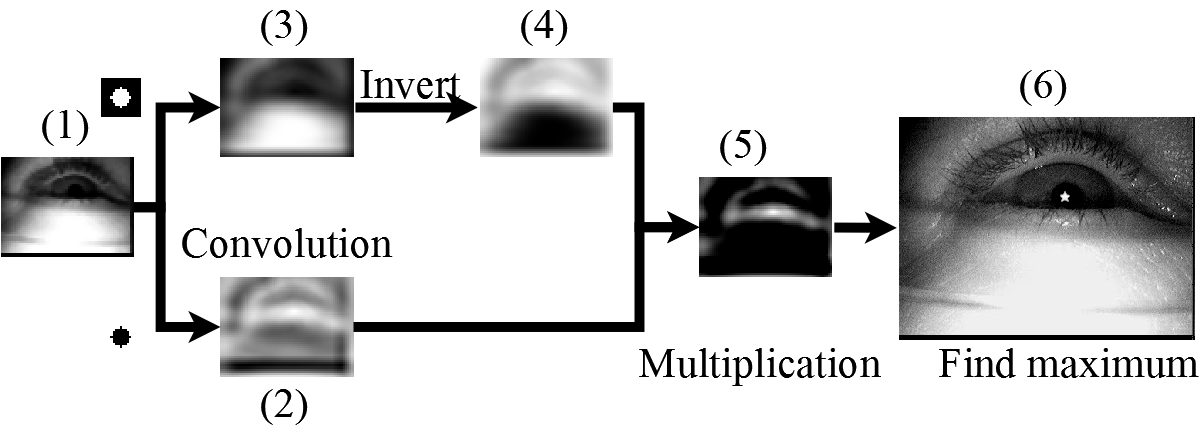
\includegraphics[width=0.8\linewidth]{img/ElSe}
	\caption{Ablauf der alternativen Berechnung zur Pupillen-Detektion}
	\label{img_else}
\end{figure}
\subsection{Ergebnisse}
Im Vergleich zu en anderen Verfahren im Test, zeig sich das ElSe in den meisten Fällen als Sieger hervorgeht mit einer Verbesserung der Erkennungsrate um $14.53\%$.\\
Ein Problem entsteht wenn der Farbunterschied zwischen Iris und Pupille recht gering ist, oder durch Reflektionen der Kantenverlauf gestört wird.\\
To DO: Quellen für Vergleich